\section{Introduction}
% Just a first sketch:
This Bachelor Thesis is about writing a fast and interactive 3D visualization environment for scientific computing. 
The focus is on usability, applied to all the different interfaces, ranging from abstract API interfaces to graphical user interfaces. 
The ultimate goal is to make scientific computing more accessible to the user.
As \ac{GUI} elements and editable text fields are supplied, one can also write and execute scripts, and immediately visualize all bound variables of the script and edit them via simple \ac{GUI} elements like sliders. 
With this it is possible to implement rudimentary interactive programming or visual debugging, further helping the user to understand his algorithms.

The introduction is structured in the following way.
First, an introduction to the general field of research and its challenges is given. 
From these challenges, the problems relevant to this thesis will be extracted.
Finally this chapter will conclude with a solution to the problem, how to measure the success and give an outlook on the structure of the entire Bachelor Thesis.
 
\subsection{Field of Research and Problem}

\vspace{1em}
\begin{minipage}{\linewidth}
    \centering
    
\includegraphics[width=0.7\linewidth]{graphics/surfaces.png}
    \captionof{figure}[Volume Visualization]{different visualizations of $f(x,y,z)=\sin(\frac{x}{15})+\sin(\frac{y}{15})+\sin(\frac{z}{15})$, visualized with Romeo. From left to right: Isosurface with isovalue=0.76, Isosurface with isovalue=0.37, maximum value projection}
    \label{fig:volume}
\end{minipage}
\vspace{1em}

%Scientific computing: visual debugging, interactive programming, high performance
%First rough sketch:
The general research field is making the capabilities of computers more accessible and understandable.
This is a very broad definition and there are many different ways of making it easier to use a computer. 
One of the first big steps was to move from coding in binary to assembly. 
Many more steps have followed, for example introducing graphical user interfaces, novel input devices like the mouse, understandable visualizations and so forth.
All these advances have made computers usable even for people who don't have an education in computer science.
In this bachelor thesis the field is scientific computing, which still has quite a lot of barriers for novel users.
Scientific computing is usually about implementing mathematical equations, complex algorithms and manipulating and analyzing data.
As it is difficult to offer easy to use graphical interfaces for this kind of work, most research is done in some specialized, high-level scientific computing language. As most high-level languages are relatively slow, but for a lot of algorithms state of the art performance is required, this has led to a dual system. Prototyping in a high-level language, and then redoing the work in a fast low-level language.
That this is not the perfect work flow is immediately visible, and a lot of research has been put into making high-level languages faster.
These efforts slowly pay off and there is a whole new range of languages, that claim to be easy to work with while being as fast as it can get.
This is a relatively recent trend and hasn't fully arrived in scientific computing yet, as most languages still have their core implemented in another fast language, which makes it hard to extend them for non professional users.
This is especially true for high performance visualization libraries, which mostly use C++ at their performance critical core.
To leverage the extensibility of these libraries, this bachelor thesis implements a visualization library in a fast high level language.
Visualizations where chosen as they're a crucial building blocks for many fields in scientific computing.

Consider the following function $f(x,y,z)=\sin(\frac{x}{15})+\sin(\frac{y}{15})+\sin(\frac{z}{15})$, which describes a 3D volume mathematically. 
This is a simple function, which is already not that easy to interpret. In figure \ref{fig:volume}, you can see different visualizations of f. 
Especially for more complex functions, visualizing might be the only way to get a deeper understanding of the values that a formula or algorithm produces.
This deeper understanding is crucial for identifying problems in the underlying math, or extending the algorithm.
Additionally, widgets and simple \ac{GUI}s are indispensable, giving scientist an easy way to interact with their data and algorithms.
This helps to further understand the dynamics of the data and quickly spot mistakes.

In summary, the software in this thesis (Romeo) focuses on research which involves writing short scripts, while playing around with some parameters and visualizing the results. 
An example would be a material researcher, who is investigating different 3D shapes and materials and their reaction to pressure.
The researcher would need to read in the 3D object he wants to analyze, have an easy way to tweak the material parameters and it would be preferable to get instant feedback on how the pressure waves propagate through the object.


\subsection{Problem Solutions and Measurements of Success}

All building blocks in this thesis are developed with the purpose in mind to give the user the possibility to visualize and interact with complex 2D and 3D data, while being able to easily extend the library.
To enable this kind of functionality, a lot of parts of the infrastructure need to work seamlessly together.
Certain design choices had to be made to guarantee this. As speed is the most constraining factor, I will start by introducing the design choices that had to be made in order to achieve state of the art speed.

\vspace{1em}
\begin{minipage}{\linewidth}
    \centering
    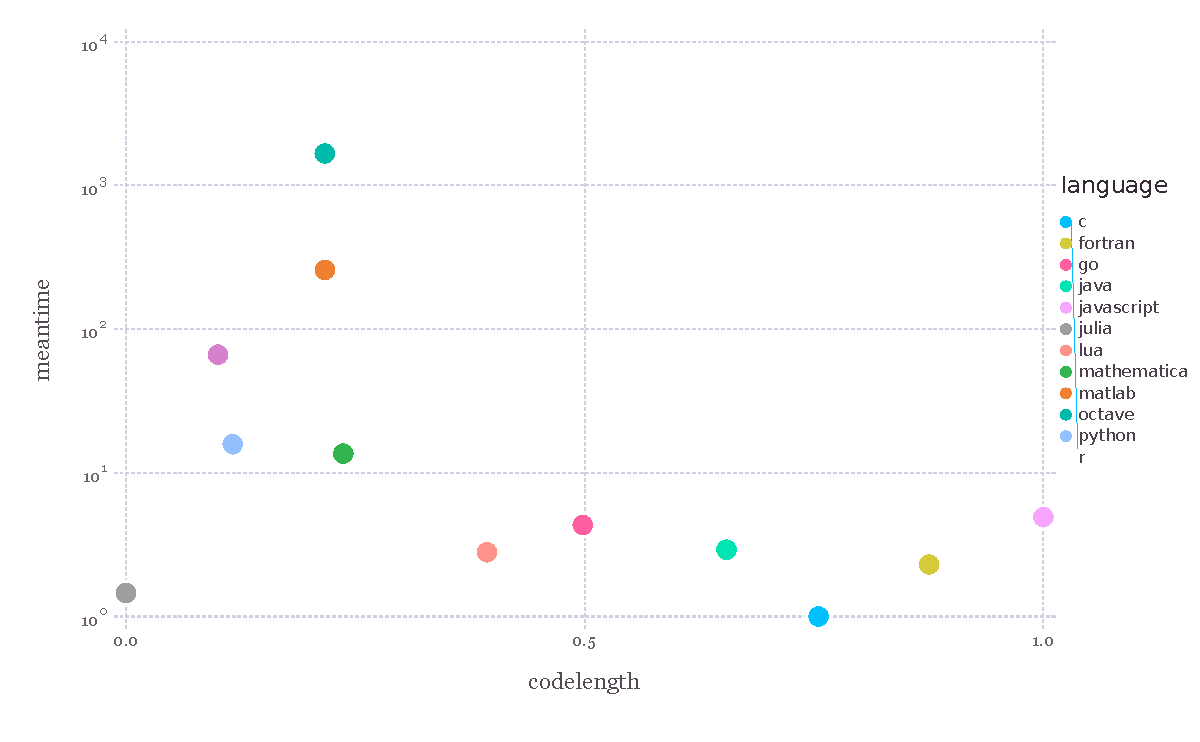
\includegraphics[width=0.9\linewidth]{graphics/julia_bench.pdf}
    \captionof{figure}[Volume Visualization]{Languages speed relative to C (averaged benchmark results), plotted against the length of the needed code (Source in Appendix)}
    \label{fig:juliabench}
\end{minipage}

\subsubsection{Speed}
Speed is mainly a usability factor. It's a factor, that can make a software unusable, or render it unproductive. Because of this, speed has taken a high priority in this thesis. As general coding productivity is also a concern, this thesis is set on using a high level language.
Historically, these two demands can't be both satisfied.
How to achieve state of the art speed with a high level language is an ongoing research and basically the holy grail of language design.
Luckily, there is a new programming language namely Julia building upon the compiler infrastructure \ac{LLVM}, promising a concise, high-level programming style, while approaching C-performance.
This is well illustrated in figure \ref{fig:juliabench}. Code length is an ambiguous measure for conciseness, but if the code is similarly refactored it is a good indicator of how many lines of code need to be written to achieve the same goal.
\ac{LLVM} is an impressive compiler infrastructure, which has front ends for different languages and back-ends for different chip architectures. 
A language designer has the task, to emit \ac{LLVM} \ac{IR}, which than gets just in time compiled and optimized to the architecture resulting in fast machine code.
\ac{LLVM}'s concept is effective, as you can accumulate state of the art optimizations in one place, making them accessible to many languages, while being able to compile to different platforms. There are x86, ARM, OpenCL and CUDA back ends. While Julia doesn't support them all, it will hopefully be possible in the future. 
\ac{LLVM} is also used by Clang, the C/C++ front end for \ac{LLVM} rivaling \ac{gcc} and it is used by Apple's programming language Swift. 
This makes \ac{LLVM} a solid basis for a programming language, as these are highly successful projects guaranteeing \ac{LLVM} further prospering of the technology.
%See table \ref{table:FEComparison}, for a little benchmark.

To get high performant 3D graphics rendering, there are on the first sight a lot of options.
If you start to take the previous demands into account, the options shrink down considerably, though.
It should be implemented in one high level language, which can be used for scientific computing and has state of the art speed. At this point, there are close to zero libraries left. As you can see in figure \ref{fig:juliabench}, Matlab, Python and R disqualify, as they are too slow. JavaScript, Java, Go and Lua are missing a scientific background and the others are too low level for the described goals.
This leaves only Julia, but in Julia there weren't any 3D libraries available, which means that one has to start from scratch.
There are only a couple of GPU accelerated low-level libraries available, namely Khrono's OpenGL, Microsoft's DirectX, Apple's Metal and AMD's Mantel, which are offering basically the same functionality. As only OpenGL is truly cross-platform, this leaves only OpenGL as an option.
So for the purpose of high speed visualizations, OpenGL was wrapped with a high-level interface written in Julia. This leaves us with one binary dependency not written in Julia, namely the video driver, which implements OpenGL.

Measurement of success is pretty straight forward, but the devil is in the detail.
It's easy to benchmark the code, but quite difficult to find a baseline, as one either has to implement the whole software with the alternative technologies, or one has to find similar software.
I will follow a hybrid strategy, comparing some simple implementations with different technologies and choose some rivaling state of the art libraries as a baseline.

\subsubsection{Extensibility}
Extensibility is an important factor, which can decide, if a library is fit for scientific computing or not. 
It's not only that, but also a great factor determining growth of a software, as the more extensible the software is, the higher the probability that someone else contributes to it.
In order to write extensible software, we first have to clarify what extensibility is.
Extensible foremost needs, that the code is accessible. There are different levels of accessibility. The lowest level is closed source, where people purposely make the code inaccessible. While this is obvious, it is just a special case of not understanding the underlying language. Just shipping binaries without open sourcing the code, means that the source is only accessible in a language which is extremely hard to understand, namely the machine code of the binary. So another example for inaccessibility is to write in a language that is difficult to understand. Other barriers are obfuscated language constructs, missing documentations and cryptic highly optimized code.
Further more the design of the library in the whole is an important factor for extensibility. It's not only important, that all parts are understandable, but also, that every independent unit in the code solves only one problem.
If this is guaranteed, re-usability in different contexts becomes much simpler. This allows for a broader user base, which in turn results in higher contributions and bug reports.
Short concise code is also important, as it will take considerably less time to rewrite something, as the amount of code that has to be touched is shorter and less time is spend on understanding and rewriting the code.

So the code written for this thesis should be open source, modular, written in a high level language and concise.

This is pretty difficult to measure as these are either binary choices, which are either followed or not, 
or higher level concepts like writing concise code, which can be a matter of taste.

\subsubsection{Event System}
For interaction events have to be handled. The chosen event system is named Reactive, which also reflects its design principle.
Reactive programming is an event driven approach, using signals as the abstraction. 
Signals are values, which change over time, which can be transformed via functions, yielding a new signal.
Here is an example to clarify the notion of signals:
\begin{lstlisting}
a = Input(40) # an integer signal.
b = Input(2) # an integer signal.
c = lift(+, a,b) # creates a new signal with the value 42
push!(a, 20) # updates a, resulting in c being 22
\end{lstlisting}

The event system was chosen for two reasons:
First, because it simply was the only available event system for Julia at that time.
Secondly, it naturally represents change over time, which is a perfect fit for animations.


\subsubsection{Interfaces}
Working with a computer means working with interfaces to a computer, which in the end simply jiggles around with zeros and ones. There is a huge hierarchy of abstractions involved, to make this process of binary juggling manageable to the human.
We already dealt with the lowest relevant abstraction: the choice of programming language, which forms our first interface to the computer.
The next level of abstraction is the general architecture of the modules, which has been discussed previously. 
This chapter is about the API design choices that have been made.
The first API is the OpenGL layer. The philosophy is to make the wrapper for native libraries as thin and reusable as possible and an one to one mapping of the library itself.
This guarantees re-usability for others, as they might be used to work only with the low-level library and they might disagree with any higher-level abstraction.
Over this sits an abstraction layer needed to simplify the work with OpenGL.
With this abstraction, the actual visualization library is implemented.
APIs for visualization libraries are very difficult to realize, as there are endless ways of visualizing the same data.
The design choice here was to use Julia's rich type system, to better describe the data. 
Julia makes this possible, as you can name the same data differently, without loosing performance.
So you can actually have a unit like meter represented as a native floating point type and have the visualization specialize to this.
Like this you can have a single function e.g. \textit{visualize}, that does creates a default visualization for a lot of common data.
It is parameterizable and can actually be overloaded for different styles.
So the signature looks like this in the end:
\begin{lstlisting}
visualization{data} = visualize(data, style=default, parameters=default)
\end{lstlisting}
The same principle is used for editing data, so there is also:
\begin{lstlisting}
visualization{data}, signal{data} = edit(data, style=default, parameters=default)
\end{lstlisting}
Together with the event system which consists of signals, it is possible to edit and visualize rich data over a simple interface, which is perfect for visual debugging, as it is always the same function call applied to the data and no further user interaction is needed.
It is also easy to extend, as the user just has to overload the function, with a custom style and or parameters.
Finally, there are also graphical user interfaces developed for this thesis. As also optimizing them is out of the scope of this thesis, they're kept very simple.
The measurement of success is again relatively difficult to do. (I need to think this over)

\subsection{Outlook}
%Structure of BA and a few worts on the results 

\subsection{Used Technologies}

\subsubsection{Julia}
\subsubsection{OpenGL}


\subsection{Similar Work}

\subsubsection{Other Languages}
\subsubsection{Ipython Notebook}
\subsubsection{Matlab}
\subsubsection{Mathematica}
\subsubsection{Other Graphic acceleration APIs}